%\documentclass[journal = jpccck, manuscript = article, layout=onecolumn]{achemso}
\documentclass[12pt]{article}
%--------------------   start of the 'preamble'
%
\usepackage{graphicx,amssymb,amstext,amsmath,color}
\usepackage[margin=2cm]{geometry}
\usepackage{abstract}
\usepackage{setspace}
\usepackage[footnotesize,bf]{caption}

% TABLE
\usepackage{multicol,hhline,colortbl,multirow}
\usepackage{braket}
\usepackage{siunitx}
\usepackage{hyperref}
\usepackage{authblk}
\usepackage{siunitx}
\usepackage{mathrsfs}
\usepackage{wrapfig}
%%\usepackage[sort&compress]{natbib}
%%\bibpunct{(}{)}{,}{a}{, }{;}
%
\usepackage[sort&compress]{natbib}
\bibpunct{[}{]}{,}{s}{}{;}


\definecolor{gray}{gray}{0.8}
\def\mobunits{\square\centi\meter\per\volt\per\second}
\def\gcm{\gram\per\cubic\centi\meter}
\def\ccg{\cellcolor{gray}}

\renewcommand{\labelitemii}{$\circ$}
\renewcommand{\bibname}{References}

\renewcommand\Affilfont{\itshape\scriptsize}

\title{Type I: Machine Learning for Structure-Performance Relationships in Organic Semiconducting Devices}
\author[1]{Matthew L. Jones}
\author[2]{Evan D. Miller}
\author[3]{Bryan Stanfill}
\author[4]{Eric Jankowski}
\affil[1]{mattyjones@boisestate.edu, Micron School of Materials Science and Engineering, Boise State University, Boise ID 83725}
\affil[2]{evanmiller326@boisestate.edu, Micron School of Materials Science and Engineering, Boise State University, Boise ID 83725}
\affil[3]{bryan.stanfill@pnnl.gov, Pacific Northwest National Laboratory, Richland WA 99354}
\affil[4]{ericjankowski@boisestate.edu, Micron School of Materials Science and Engineering, Boise State University, Boise ID 83725}

%%\affiliation{Micron School of Materials Science and Engineering, Boise State University, Boise ID 83725}
%%\email{mattyjones@boisestate.edu}
%\author{Evan D. Miller}
%%\affiliation{Micron School of Materials Science and Engineering, Boise State University, Boise ID 83725}
%%\email{evanmiller326@boisestate.edu}
%\author{Bryan Stanfill}
%%\affiliation{Pacific Northwest National Laboratory, Richland WA 99354}
%%\email{bryan.stanfill@pnnl.gov}
%\author{Eric Jankowski}
%%\affiliation{Micron School of Materials Science and Engineering, Boise State University, Boise ID 83725}
%%\email{ericjankowski@boisestate.edu}
\date{}

\begin{document}
\maketitle

%\begin{figure}[h!]\centering
%	\includegraphics[width=0.5\textwidth]{Figures/PublishedHoleMob.pdf}
%    \caption{The mobility trend observed as a function of increasing temperature}
%	\label{fig:MSD}
%\end{figure}

The goal of the proposed work is to understand electron and hole transport in organic semiconductors, enabling the mitigation of global climate change through the production of high-efficiency, low cost solar panels. 
The challenge we address here is understanding how the chemistry and packing of photoactive molecules affects the motion of electrons and holes in the organic active layer.
Ordinarily, this investigation requires the execution of a large number of slow quantum chemical calculations to predict the electronic properties of the materials.
This demands excessive computing power, limiting the exploration of the vast phase space of different chemistries and processing statepoints, and prohibiting the identification of actionable design rules for the manufacturing of efficient devices.
Our hypothesis is that machine learning techniques, trained on a small subset of quantum chemical data, can be used to predict the electronic capabilities of nanostructure morphologies to dramatically reduce the number of expensive calculations to be performed and facilitate high-throughput parameter-sweep studies of candidate chemistries and processing.


Organic semiconductors are becoming an increasing popular alternative to conventional inorganics in the construction of electronic devices\cite{Tsumura1986,Friend1999,Sariciftci1992} thanks to recent advances in synthetic chemistry and scalability of low-cost manufacturing processes.
However, the efficiency of organic devices (and particularly organic photovoltaics) tends to be significantly lower than conventional devices.
In particular, the charge-carrier mobility describes the speed at which electrons and holes can move through the active layer of the device, and is a crucial factor in device efficiency\cite{Sirringhaus2014}.
The mobility often depends sensitively on the morphology of the active layer, which describes the relative positions and orientations of the component molecules.
Therefore, in order to manufacture the most efficient devices, it is vital to optimize the morphology such that the charge-carrier mobility is maximized.
The molecular morphology can be influenced by the choices of chemistries in the system, as well as the device processing conditions such as temperature, pressure, solvent choice, and annealing duration\cite{Noriega2013}.
This massive phase space necessitates the use of computational methods (rather than manufacturing hundreds of millions of test devices in a wet lab) that are capable of spanning multiple length- and time-scales.

\clearpage
\begin{wrapfigure}{lb}{0.5\textwidth}\centering
%\begin{figure}[h!]\centering
%\vspace{1em}
	\includegraphics[width=0.5\textwidth]{Figures/fig.png}
    %\begin{tabular}{cc}
    %    \includegraphics[width=0.5\textwidth]{Figures/morphologySpam.png} &
	%    \includegraphics[width=0.5\textwidth]{Figures/flowchartFull.png}
    %\end{tabular}
    \caption{Predicting charge mobility for a single simulation snapshot requires quantum chemical calculations be performed on each pair of chromophores. Machine learning techniques represent a way to obtain electronic transfer integrals between chromophore pairs, saving potentially billions of unnecessary, expensive chemical calculations per semiconductor study.}
	\label{fig:fig1}
%\end{figure}
\end{wrapfigure}

Carriers move through the morphology via quantised tunnelling events - `hops' - between electronically active functional groups on the molecules known as `chromophores'.
The rate at which a carrier hop can occur from chromophore $i$ to chromophore $j$, $k_{ij}$, is given by the semi-classical Marcus expression\cite{Marcus1964}:
\begin{equation}\label{eq:Marcus}
    k_{ij} = \frac{\left| T_{ij} \right|^{2}}{\hbar} \sqrt{\frac{\pi}{\lambda k_{B} T}} \exp \left[ - \frac{(\Delta E_{ij} + \lambda)^{2}}{4 \lambda k_{B} T} \right],
\end{equation}
where $T_{ij}$ is the electronic transfer integral, $\Delta E_{ij}$ is the difference in energy between the initial and final hop sites, and the remaining parameters are material-specific, thermodynamic or fundamental constants.
The speed at which a hop from one chromophore to a neighbour can occur is primarily governed by $T_{ij}$, which is a measure of the amount of molecular orbital overlap between the pair.
%A large transfer integral describes an easy hop, which can happen quickly, leading to a fast charge carrier, a high carrier mobility, and a more efficient device.

Current state-of-the-art predictions of mobility combine computational techniques: molecular dynamics simulations to obtain a candidate morphology, quantum chemical calculations to determine the transfer integrals and hop rates between chromophores, and kinetic Monte Carlo to simulate charge motion through the device (Figure \ref{fig:fig1})\cite{MorphCT,Jones2016,Jones2017}.
These simulations can take several days to run on supercomputers even with GPU acceleration hardware for just a single selection of component molecules and device processing techniques.
Optimizing the simulation pipeline will dramatically improve computational throughput of the screening process required to detect combinations of molecules and processing that will result in the most efficient devices.
One area of opportunity we have identified is the calculation of transfer integrals via quantum chemical calculations: of the 1,000-100,000 chromophore pairs that make up a single simulation snapshot, many pairs share the same local structure and therefore have the same transfer integrals.
Performing quantum chemical calculations for each pair of chromophores therefore represents an inefficiency compared to a sufficiently accurate pattern recognition scheme that can look up transfer integrals based on their local structure.

We propose using machine learning techniques to streamline the quantum chemical portion of the pipeline by predicting carrier transfer integrals between pairs of chromophores.
Our preliminary work has investigated a semi-crystalline test system containing 1,000 oligomers of poly(3-hexylthiophene), each of length 15 monomers.
For each pair of nearest-neighbour monomers, we use semi-empirical quantum chemical calculations to predict the electronic transfer integrals, for a total of 40,000 data points.
In general, monomers are defined by the locations of their constituent atoms and bonds, and the transfer integral can be determined by considering the relative position of each monomer to its neighbour.
As such, we consider only geometric descriptors for each pair, constructured from 6 independent labels corresponding to relative translations in three dimensions, and relative rotations around three orthogonal axes.
We explored the efficacy of linear models (such as splines and regression), as well as artificial neural networks and kernel-based methods (support vector machines) in predicting the transfer integrals, each of which were trained using a selection of the 40,000 data points.
Of the methods explored, random-forest decision tree techniques provided the most accurate, resulting in a correlation coefficient of $r^{2} = 0.976$, corresponding to an average absolute error of 34 meV, far below the expected 100 meV accuracy of even the most computationally intensive quantum chemical predictions.
\textcolor{red}{$<$I expect Bryan will have more to say about this section$>$}

\subsection{Why is a continuation warranted and promising?}

The small average errors in our models prediction is extremely promising for machine learning techniques to be able to evaluate tens of thousands of \textit{in situ} in a matter of minutes instead of days.
\begin{wrapfigure}{lb}{0.5\textwidth}\centering
	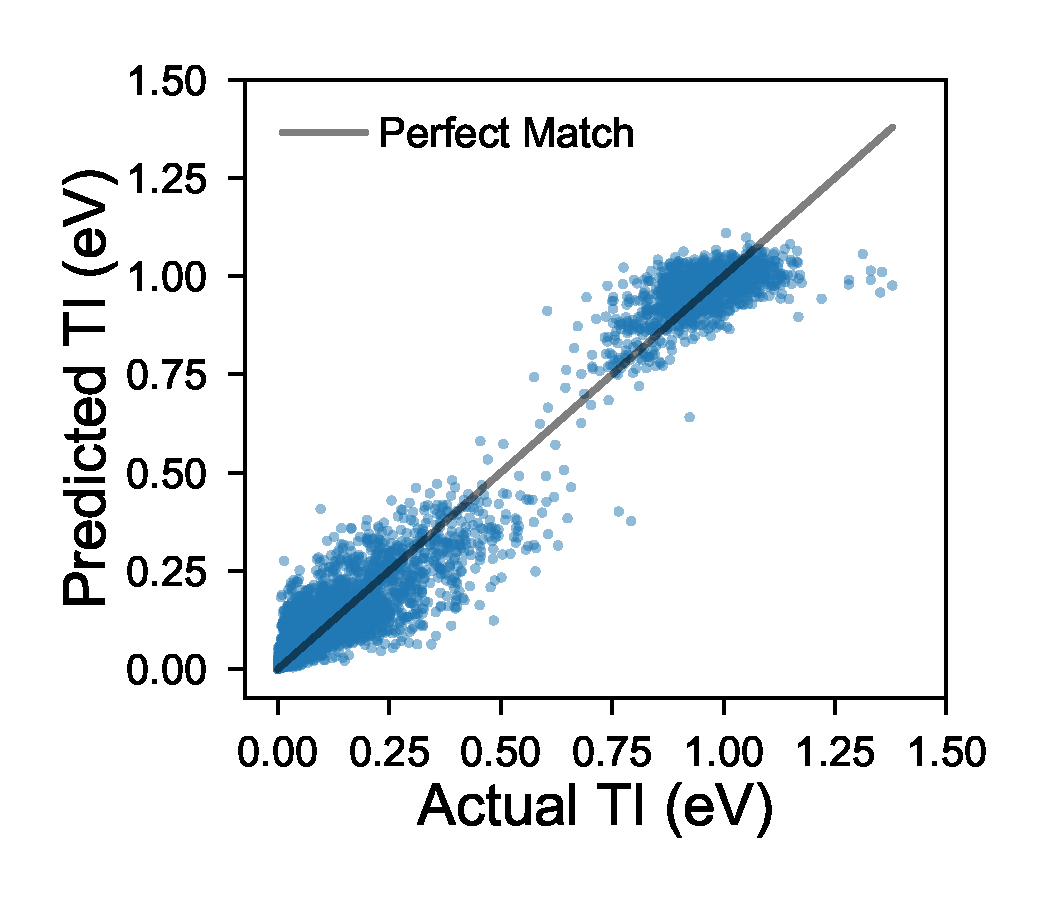
\includegraphics[width=0.5\textwidth]{Figures/comparison.pdf}
    \caption{
The comparison of the transfer integrals calculated by ZINDO/S compared to those predicted by the random forest.
This produces an average absolute error of 30 meV and an $R^2$ value of 0.978.
}
	\label{fig:random_forest_results}
%\end{figure}
\end{wrapfigure}
Figure \ref{fig:random_forest_results} shows that optimisations to our model can still be made.
We intend to explore more combinations of descriptors to tighten up the model and reduce the average error by still further, to a target value of 10 meV.


\subsection{What could be achieved with additional resources?}


\subsection{Why is this important to materials research?}

\subsection{Why is this important to data science?}

\subsection{Budget}

\subsection{External data resources and cyberinfrastructure}


Neural networks are an especially promising candidate due to their efficient parallelizability to be executed on GPUs, bringing the rest of the simulation pipeline in line with the molecular dynamics simulations\cite{Oh2004}.
We will train our model using the wealth of data already obtained from the pipeline and by providing key structural descriptors such as position and orientation of chromophore pairs in the system, and then measure its accuracy in predicting transfer integrals for preliminary data left out of the training set.
We also aim to train a separate network to predict the relative deviations in energy levels between chromophores to obtain the $\Delta E_{ij}$ term in equation \ref{eq:Marcus}, effectively replacing both of the slowest components of the pipeline.

The current dataset to be used for training and testing consists of around 500 unique morphologies, covering 10 chemistries including polymers, fullerenes, block co-polymers and polycyclic aromatic hydrocarbons, each with at least 3 processing state points above and 3 state points below an order-disorder transition temperature for each chemistry.
Each morphology contains, on average, 100,000 atoms resulting in $\sim$20,000 chromophore pairs per morphology.
Each pair creates an output file in text format, with size $\sim$50 KB, describing the 3-dimensional positions of the constituent atoms as well as the scalar molecular orbital energies.
In total, we have already generated electronic properties data for over 10,000,000 chromophore pairs, corresponding to several hundreds of GB of raw data.
All data was generated using the open source MorphCT\cite{MorphCT,Jones2017}, HOOMD-Blue\cite{Anderson08}, and ORCA\cite{Neese2012b} software suites and will be made freely available through digital hosting provided by the Albertsons Library at Boise State University.

\newpage


\bibliography{refs}
\bibliographystyle{unsrt}

\end{document}
